%% LaTeX-Beamer template for KIT design
%% by Erik Burger, Christian Hammer
%% title picture by Klaus Krogmann
%%
%% version 2.1
%%uage
%% mostly compatible to KIT corporate design v2.0
%% http://intranet.kit.edu/gestaltungsrichtlinien.php
%%
%% Problems, bugs and comments to
%% burger@kit.edu

\documentclass[18pt]{beamer}

%% SLIDE FORMAT

% use 'beamerthemekit' for standard 4:3 ratio
% for widescreen slides (16:9), use 'beamerthemekitwide'

\usepackage{templates/beamerthemekit}
% \usepackage{templates/beamerthemekitwide}

\usepackage[utf8]{inputenc} 
\usepackage{spreadtab}
\usepackage{multirow}
\usepackage{tikz}
\usetikzlibrary{arrows}
\usetikzlibrary{trees}
\usetikzlibrary{shapes}
\usetikzlibrary{chains}
\usetikzlibrary{calc}
\usetikzlibrary{positioning}

\usepackage[encapsulated]{CJK}
\newcommand{\cntext}[1]{\begin{CJK}{UTF8}{gbsn}#1\end{CJK}}
\newcommand{\ul}[1]{{\color{red}{#1}}}
\newcommand\Hstrut{\rule{1ex}{0pt}}

%% TITLE PICTURE

% if a custom picture is to be used on the title page, copy it into the 'logos'
% directory, in the line below, replace 'mypicture' with the 
% filename (without extension) and uncomment the following line
% (picture proportions: 63 : 20 for standard, 169 : 40 for wide
% *.eps format if you use latex+dvips+ps2pdf, 
% *.jpg/*.png/*.pdf if you use pdflatex)

%\titleimage{mypicture}

%% TITLE LOGO

% for a custom logo on the front page, copy your file into the 'logos'
% directory, insert the filename in the line below and uncomment it

%\titlelogo{mylogo}

% (*.eps format if you use latex+dvips+ps2pdf,
% *.jpg/*.png/*.pdf if you use pdflatex)

%% TikZ INTEGRATION

% use these packages for PCM symbols and UML classes
% \usepackage{templates/tikzkit}
% \usepackage{templates/tikzuml}

% the presentation starts here

%\title[Short title]{Analyzing the Potential of Source Sentence Reordering in SMT for Chinese}
%\subtitle{Multi-Level-Tree Rule Based Preordering Approach}

\title{Rule-Based Reordering on Multiple Syntactic Levels in SMT}
%\subtitle{}
\author{Ge Wu}

\institute{Institute for Anthropomatics and Robotics (IAR)}

% Bibliography
\usepackage{csquotes} 
\usepackage[citestyle=authoryear,bibstyle=numeric,hyperref,backend=bibtex]{biblatex}
\addbibresource{folien.bib}
\bibhang1em

\setbeamercolor{alerted text}{fg=red} 
\setbeamercovered{transparent=0}
\setbeamertemplate{caption}{\raggedright\insertcaption\par}

\begin{document}

% change the following line to "ngerman" for German style date and logos
\selectlanguage{english}

%title page
\begin{frame}
\titlepage
\end{frame}

%table of contents
\begin{frame}{Outline}
\tableofcontents
\end{frame}

\section{Introduction}
\begin{frame}{Introduction}
%Goal \& Motivation \& Reason, etc.
\begin{itemize}
\item Rule-based pre-ordering approaches {\scriptsize [\cite{short, long, tree}]}
\item Hierarchical phrase-based model {\scriptsize [\cite{hier}]}
\item More adaptive pre-ordering approach for Chinese based on syntactic structures
\end{itemize}
\end{frame}

%\subsection{System}
\begin{frame}{Pre-ordering System}
\begin{figure}
\centering
\newlength\mylens
\setlength{\mylens}{1cm}

\begin{tikzpicture}[scale=0.7,
->,>=stealth', grow=right, level 1/.style={sibling distance=1.3\mylens}, level distance=4\mylens,
node/.style = {scale=0.7, align=center, inner sep=0pt, text centered, font=\sffamily, rectangle, rounded corners, draw=black, thick, fill=blue!20, text width=5em, minimum height = 2em, inner sep=5},
nodeimp/.style = {node, fill=red!20},
lab/.style={scale=0.7}
]


\node(A) [node, text width=8em] at (0, 0) {Source Sentences};
%\node(B) [node, below=\mylens of A] {Reordering};
\node(B) [draw=black, thick, circle, below=\mylens of A] {};
\node(C) [node, text width=8em, text height=4ex, below=2\mylens of B] {Decoder\\ \vphantom{x}};

\node (CW) [left=1pt of C.south west] {};
\node (CE) [right=1pt of C.south east] {};
%\draw[-, line width=10pt, white] (CW) to (CE);
%\node(XX) [below=0.1\mylens of C] {};
%\node(X) [node, draw=white, rounded corners=0, fill=white, maximum height = 0.1em] at (C.south) {};

\node(E) [nodeimp, right=1.4\mylens of B] {Reordering Rules};
\node(EE) [draw=black, thick, circle, right=1.6\mylens of E] {};

\node(F) [nodeimp, above right=0.3*\mylens and 2.85\mylens of E] {Word Alignment};
\node(G) [nodeimp, right=2.85\mylens of E] {POS Tags};
\node(H) [nodeimp, below right=0.3*\mylens and 2.85\mylens of E] {Syntactic Tree};

\node(I) [node, right=\mylens of G] {Training Data};


\draw[->, thick] (A) to (B);
\draw[white] (C) to node[lab, black, midway, sloped, above] {Lattices} (B);
\draw[->, thick] (B) to (C);
\draw[->, thick] (E) to node[lab, midway, above] {Apply} (B);
\draw[->, thick] (EE) to node[lab, midway, above] {Extract} (E);

\node(Saa) [right=0.5\mylens of EE] {};
\node(Sbb) [left=0.5\mylens of I] {};

\coordinate(Sa) at (Saa.base);
\coordinate(Sb) at (Sbb.base);

\draw[->, thick] (Sa) to (EE);
\draw[-, thick] (I) to (Sb);

\draw[-, thick] (F.west) -| (Sa);
\draw[-, thick] (G.west) -| (Sa);
\draw[-, thick] (H.west) -| (Sa);

\draw[->, thick] (Sb) |- (F.east);
\draw[->, thick] (Sb) |- (G.east);
\draw[->, thick] (Sb) |- (H.east);

%\node(2) [below=1cm of A, node, minimum height = 10 em] at (0\myxa,3\myya) {Decoder};
%\node(3) [node] at (0\myxa,2\myya) {Target Sentences};


%\node(1) [nodeimp] at (3\myxa,4\myya) {Reordering Rules};

%\draw[->] (0) to node [midway, sloped, below] {} node [midway, sloped, above] {} (1);

\end{tikzpicture}
%\caption{Preordering system}
%\label{prereordering}
\end{figure}
\end{frame}


%\subsection{Reordering Rules}
\begin{frame}{Reordering Rules}
\begin{itemize}[<+-| alert@+>]
\setbeamerfont{alerted text}{series=\bfseries}
\setbeamercolor{alerted text}{fg=black} 
\item Short rules {\scriptsize [\cite{short}]}
\item Long rules {\scriptsize [\cite{long}]}
\item Tree rules {\scriptsize [\cite{tree}]}
\end{itemize}
\begin{overprint}
\onslide<1>
\begin{itemize}
\item[] 
\begin{itemize}
\item[] \texttt{after the accident -> the accident after (0.5)}\bigskip \\
\item[] \texttt{WRB MD DT -> DT WRB DT (0.3)}
\end{itemize}
\end{itemize}
\onslide<2>
\begin{itemize}
\item[] 
\begin{itemize}
\item[] \texttt{NN * MD -> * MD NN (0.14)}
\end{itemize}
\end{itemize}
\onslide<3>
\begin{itemize}
\item[] 
\begin{itemize}
\item[] \texttt{NP ( ADJP JJ NN ) -> JJ NN ADJP (0.16)}
\end{itemize}
\end{itemize}
\begin{figure}
\centering
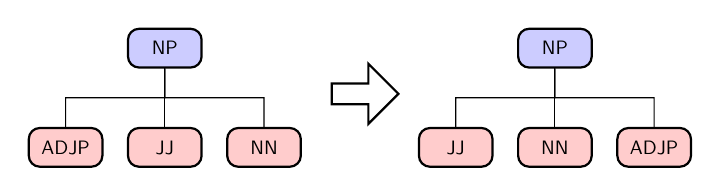
\begin{tikzpicture}[scale=0.7,
-,>=stealth',
level/.style={sibling distance = 1.8cm, level distance = 1.8cm},
%level 1/.style={sibling distance=8cm},
%level 2/.style={sibling distance=4cm}, 
%level 3/.style={sibling distance=4cm}, 
treenode/.style = {scale=0.7,align=center, minimum width=3.8em, minimum height = 2em, inner sep=0pt, text centered, font=\sffamily},
arn_n/.style = {treenode, rectangle, rounded corners, draw=black, thick, fill=blue!20},
arn_x/.style = {arn_n, fill=red!20},
edge from parent fork down
]
\node (A) [arn_n] {NP}
child{ node [arn_x] {ADJP}}
child{ node [arn_x] {JJ}}
child{ node (X) [arn_x] {NN}};



\node (B) [arn_n, right = 4cm of A] {NP}
child{ node (Y) [arn_x] {JJ}}
child{ node [arn_x] {NN}}
child{ node [arn_x] {ADJP}};

\node (XX) [below right=0.2cm and 0.5cm of A] {};
\node (YY) [below left= 0.2cm and 0.5cm of B] {};


%\draw[-,double distance=2pt] (XX) to (YY);
%\draw[open triangle 60, thick] (XX) to (YY);
\draw[draw=none] (XX) to node[draw, thick, midway, single arrow] {\Hstrut\Hstrut\Hstrut} (YY);
\end{tikzpicture}


\end{figure}
\end{overprint}
\end{frame}


%\subsection{Chinese Word Orders}
\begin{frame}{Chinese Word Orders}
\begin{itemize}[<+-| alert@+>]
\setbeamerfont{alerted text}{series=\bfseries}
\setbeamercolor{alerted text}{fg=black} 
\item Pre-modifier instead of post-modifier
\item Questions
\item Special sentence constructions
\item Long distance position change
\end{itemize}
\begin{overprint}
\onslide<1>
\vspace{-2cm}
\begin{itemize}
\item[]
\begin{itemize}
	\item Adverbials
	\item Relative clauses
	\item Preposition phrases
\end{itemize}
\end{itemize}	
%\vspace{-1cm}
\begin{figure}
\centering
\begin{tikzpicture}[
node/.style = {
text centered, 
text height=1.5ex,
text depth=.25ex,
inner sep=2pt, font=\sffamily, rectangle, draw=none, fill=none, outer sep=0,
minimum height=4ex
},
node2/.style = {
text height=4.25ex, text depth=.25ex, draw=black, inner sep=0, outer sep=0, rounded corners
},
]

\node(A1) [node] at (0, 2.5) {Those};
\node(A2) [node, right=1em of A1] {are};
\node(A3) [node, right=1em of A2] {conveyor};
\node(A4) [node, right=1em of A3] {belts};
\node(Ax) [node2, right=1em of A4] {
\tikz\node(A5) [node] {that};
\tikz\node(A6) [node, right=1em of A5] {go};
\tikz\node(A7) [node, right=1em of A6] {around};
};
\node(A8) [node, right=1em of Ax] {.};

\node(B1) [node] at (0, 0) {\cntext{那些}};
\node(B2) [node, right=2.475em of B1] {\cntext{是}};
\node(Bx) [node2, right=2.475em of B2] {
\tikz\node(B3) [node] {\cntext{在}};
\tikz\node(B4) [node, right=2.475em of B3] {\cntext{运转}};
\tikz\node(B5) [node, right=2.475em of B4] {\cntext{的}};
};
\node(B6) [node, right=2.475em of Bx] {\cntext{传送带}};
\node(B7) [node, right=2.475em of B6] {\cntext{。}};

%1-1 2-2 3-6 4-6 5-6 6-6 7-6 8-7

\draw[dashed] (A1.south) -- (B1.north);
\draw[dashed] (A2.south) -- (B2.north);
\draw[dashed] (Ax.south) -- (Bx.north);
\draw[dashed] (A3.south) -- (B6.north);
\draw[dashed] (A4.south) -- (B6.north);
\draw[dashed] (A8.south) -- (A8|-B7.north);
\end{tikzpicture}

\end{figure}
\onslide<2>
\vspace{-1.2cm}
\begin{figure}
\centering
\begin{tikzpicture}[
node/.style = {
text centered, 
text height=1.5ex,
text depth=.25ex,
inner sep=2pt, font=\sffamily, rectangle, draw=none, fill=none, outer sep=0,
minimum height=4ex
},
node2/.style = {
text height=4.25ex, text depth=.25ex, draw=black, inner sep=0, outer sep=0, rounded corners
},
]

\node(A1) [node] at (0, 2) {How};
\node(A2) [node, right=1em of A1] {will};
\node(A3) [node, right=1em of A2] {you};
\node(A4) [node, right=1em of A3] {cook};
\node(A5) [node, right=1em of A4] {the};
\node(A6) [node, right=1em of A5] {chicken};
\node(A7) [node, right=1em of A6] {?};

\node(B1) [node] at (0, 0) {You};
\node(B2) [node, right=1.23em of B1] {will};
\node(B3) [node, right=1.23em of B2] {\alert{how}};
\node(B4) [node, right=1.23em of B3] {cook};
\node(B5) [node, right=1.23em of B4] {chicken};
\node(B6) [node, right=1.23em of B5] {};
\node(B7) [node, right=1.23em of B6] {?};

\node(C1) [node, below=0 of B1.south] {\cntext{你}};
\node(C2) [node, below=0 of B2.south] {\cntext{会}};
\node(C3) [node, below=0 of B3.south] {\cntext{\alert{怎么}}};
\node(C4) [node, below=0 of B4.south] {\cntext{做}};
\node(C5) [node, below=0 of B5.south] {\cntext{鸡肉}};
\node(C6) [node, below=0 of B6.south] {\cntext{\alert{呢}}};
\node(C7) [node, below=0 of B7.south] {\cntext{?}};


%7-1 3-2 2-3 1-4 4-5 6-6 8-7 8-8\
\draw[dashed] (A3.south) -- (B1.north);
\draw[dashed] (A2.south) -- (B2.north);
\draw[dashed] (A1.south) -- (B3.north);
\draw[dashed] (A4.south) -- (B4.north);
\draw[dashed] (A6.south) -- (B5.north);
\draw[dashed] (A7.south) -- (B6.north);
\draw[dashed] (A7.south) -- (A7|-B7.north);

\end{tikzpicture}

\end{figure}
\onslide<3>
\begin{itemize}
\item[]
\begin{itemize}
\item[] \textit{\alert{There aren't} many people around that are really involved with architecture as clients.} \bigskip \\
\item[] \textit{\alert{Never would} India have thought on this scale before.}
\end{itemize}
\end{itemize}
\onslide<4>
\begin{itemize}
\item[]
\begin{itemize}
\item[] \textit{I find this very much disturbing \alert{when we are talking about what is going on right and wrong with democracy these days}.} \bigskip \\
\item[] \cntext{\alert{现在,每当我跟别人讨论我们的民主什么是对的,什么是错的}我都为此觉得很无力。}
\end{itemize}
\end{itemize}
\end{overprint}
\end{frame}


\section{Multi-Level-Tree (MLT) Reordering}
\subsection{Extension of tree rule based reordering to multiple syntactic levels}
\begin{frame}{Reordering on multiple syntactic levels}

\tikzstyle{treenode} = [align=center, inner sep=0.5em, text centered, font=\sffamily, scale=0.65, rectangle, rounded corners=2pt, draw=black, thick, minimum width=4em]

\tikzstyle{rr} = [treenode, fill=red!20]
\tikzstyle{r} = [treenode, fill=green!20]

\tikzstyle{n1} = [treenode, fill=blue!20]
\tikzstyle{n2} = [treenode, fill=blue!20]
\tikzstyle{n3} = [treenode, fill=blue!20]
\tikzstyle{n4} = [treenode, fill=blue!20]
\tikzstyle{n5} = [treenode, fill=blue!20]
\tikzstyle{n6} = [treenode, fill=blue!20]
\tikzstyle{n7} = [treenode, fill=blue!20]
\tikzstyle{n8} = [treenode, fill=blue!20]
\tikzstyle{n9} = [treenode, fill=blue!20]

Extension of tree rule based reordering to multiple syntactic levels 
\begin{figure}
\centering
\begin{tikzpicture}[scale=0.5,
-,>=stealth',
level/.style={sibling distance = 4cm, level distance = 1.8cm},
level 1/.style={sibling distance=7cm},
level 2/.style={sibling distance=3cm}, 
arn_z/.style = {scale=0.75},
edge from parent fork down
]

\node [n1](N1) {NP}
child{ node [n2](N2) {NP}
child{ node [n4](N4) {JJ\\ physiological}}
child{ node [n5](N5) {NNS\\ effects}}}
child{ node [n3](N3) {PP}
child[sibling distance=6cm]{ node [n6](C)(N6) {IN\\ of}}
child{ node [n7](N7) {NP}
child{ node [n8](N8) {JJ\\ environmental}}
child{ node [n9](N9) {NNS\\ hormones}}}};

\node[arn_z, below=2cm of N4](E) {\cntext{环境}};
\node[arn_z, right=0.75cm of E](F) {\cntext{荷尔蒙}};
\node[arn_z, right=0.75cm of F](G) {\cntext{的}};
\node[arn_z, right=0.75cm of G](H) {\cntext{生理}};
\node[arn_z, right=0.75cm of H](I) {\cntext{效应}};
\node[below=0.8cm of N4](J) {};
\draw[dashed] (N4)--(J)--(H.north);
\draw[dashed] (N5)--(N5|-J)--(I.north);
\draw[dashed] (N6)--(N6|-J)--(G.north);
\draw[dashed] (N8)--(N8|-J)--(E.north);
\draw[dashed] (N9)--(N9|-J)--(F.north);
\end{tikzpicture}


\end{figure}
\end{frame}

\begin{frame}{Reordering Patterns}

\tikzstyle{treenode} = [align=center, inner sep=0.5em, text centered, font=\sffamily, scale=0.65, rectangle, rounded corners=2pt, draw=black, thick, minimum width=4em]

\tikzstyle{rr} = [treenode, fill=red!20]
\tikzstyle{r} = [treenode, fill=green!20]

\tikzstyle{n1} = [treenode, fill=blue!20]
\tikzstyle{n2} = [treenode, fill=blue!20]
\tikzstyle{n3} = [treenode, fill=blue!20]
\tikzstyle{n4} = [treenode, fill=blue!20]
\tikzstyle{n5} = [treenode, fill=blue!20]
\tikzstyle{n6} = [treenode, fill=blue!20]
\tikzstyle{n7} = [treenode, fill=blue!20]
\tikzstyle{n8} = [treenode, fill=blue!20]
\tikzstyle{n9} = [treenode, fill=blue!20]

\only<2,3,4>{\tikzset{n1/.style={r}}}

\only<2>{\tikzset{n2/.style={rr}}}
\only<3,4,5>{\tikzset{n2/.style={r}}}

\only<2>{\tikzset{n3/.style={rr}}}
\only<3,4,6,7>{\tikzset{n3/.style={r}}}

\only<3,4,5>{\tikzset{n4/.style={rr}}}

\only<3,4,5>{\tikzset{n5/.style={rr}}}

\only<3,4,6,7>{\tikzset{n6/.style={rr}}}

\only<3,6>{\tikzset{n7/.style={rr}}}
\only<4,7,8>{\tikzset{n7/.style={r}}}

\only<4,7,8>{\tikzset{n8/.style={rr}}}

\only<4,7,8>{\tikzset{n9/.style={rr}}}
\vspace{-0.2cm}
\begin{figure}
\centering
\begin{tikzpicture}[scale=0.5,
-,>=stealth',
level/.style={sibling distance = 3cm, level distance = 1.5cm},
level 1/.style={sibling distance=7cm},
level 2/.style={sibling distance=3cm}, 
arn_z/.style = {scale=0.65},
edge from parent fork down
]

\node [n1,label=right:{\scriptsize 1}](N1) {NP}
child{ node [n2,label=left:{\scriptsize 2}](N2) {NP}
child{ node [n4,label=below left:{\scriptsize 4}](N4) {JJ\\ physiological}}
child{ node [n5,label=below right:{\scriptsize 5}](N5) {NNS\\ effects}}}
child{ node [n3,label=right:{\scriptsize 3}](N3) {PP}
child[sibling distance=6cm]{ node [n6,label=right:{\scriptsize 6}](C)(N6) {IN\\ of}}
child{ node [n7,label=right:{\scriptsize 7}](N7) {NP}
child{ node [n8,label=left:{\scriptsize 8}](N8) {JJ\\ environmental}}
child{ node [n9,label=right:{\scriptsize 9}](N9) {NNS\\ hormones}}}};

\node[arn_z, below=1.6cm of N4](E) {\cntext{环境}};
\node[arn_z, right=0.75cm of E](F) {\cntext{荷尔蒙}};
\node[arn_z, right=0.75cm of F](G) {\cntext{的}};
\node[arn_z, right=0.75cm of G](H) {\cntext{生理}};
\node[arn_z, right=0.75cm of H](I) {\cntext{效应}};
\node[below=0.8cm of N4](J) {};
\draw[dashed] (N4)--(J)--(H.north);
\draw[dashed] (N5)--(N5|-J)--(I.north);
\draw[dashed] (N6)--(N6|-J)--(G.north);
\draw[dashed] (N8)--(N8|-J)--(E.north);
\draw[dashed] (N9)--(N9|-J)--(F.north);
\end{tikzpicture}


\end{figure}
\vspace{-0.6cm}
\begin{itemize}
\setlength{\itemsep}{0pt}
\setlength{\parskip}{0pt}
\setlength{\parsep}{0pt}
\scriptsize
\item[] \texttt{Root Depth Pattern}
\item[]<2-> \texttt{1\hphantom{xxxx}1\hphantom{xxxxx}NP ( \ul{NP$_0$} \ul{PP$_1$} ) -> 1 0}
\item[]<3-> \texttt{1\hphantom{xxxx}2\hphantom{xxxxx}NP ( NP ( \ul{JJ$_0$} \ul{NNS$_1$} ) PP ( \ul{IN$_2$} \ul{NP$_3$} ) ) -> 3 2 0 1}
\item[]<4-> \texttt{1\hphantom{xxxx}3\hphantom{xxxxx}NP ( NP ( \ul{JJ$_0$} \ul{NNS$_1$} ) PP ( \ul{IN$_2$} NP ( \ul{JJ$_3$} \ul{NNS$_4$} ) ) ) -> 3 4 2 0 1}
\item[]<6-> \texttt{3\hphantom{xxxx}1\hphantom{xxxxx}PP ( \ul{IN$_0$} \ul{NP$_1$} ) -> 1 0}
\item[]<7-> \texttt{3\hphantom{xxxx}2\hphantom{xxxxx}PP ( \ul{IN$_0$} NP ( \ul{JJ$_1$} \ul{NNS$_2$} ) ) -> 1 2 0}
\end{itemize}
\end{frame}

\setbeamercovered{transparent=40}
\begin{frame}{Rule Extraction}
\begin{itemize}[<+-| alert@+>]
\setbeamerfont{alerted text}{series=\bfseries}
\setbeamercolor{alerted text}{fg=black} 
\item Search from all internal nodes with all possible depths
\item Rule probability
\bigskip \\
%\texttt{ADJP ( JJ , JJ ) -> 0 1 2 \hphantom{xx}  [0.84239130 = 310 / 368]}\\
\texttt{ADJP ( JJ , JJ ) -> 0 2 1 \hphantom{xx}  [0.02989130 = \hphantom{x}11 / 368]}\\
\texttt{ADJP ( JJ , JJ ) -> 1 0 2 \hphantom{xx}  [0.07880435 =  \hphantom{x}29 / 368]}\\
\texttt{ADJP ( JJ , JJ ) -> 1 2 0 \hphantom{xx}  [0.02173913 =  \hphantom{xx}8 / 368]}\\
\texttt{ADJP ( JJ , JJ ) -> 2 0 1 \hphantom{xx}  [0.02717391 =  \hphantom{x}10 / 368]} \bigskip \\
\item Rule pruning
\item Rule number doubles in comparison with tree rules
\end{itemize}
\end{frame}

\begin{frame}{Rule Application}
\begin{itemize}[<+-| alert@+>]
\setbeamerfont{alerted text}{series=\bfseries}
\setbeamercolor{alerted text}{fg=black} 
\item Search from all internal nodes with all possible depths
\item Search depth decreases to avoid duplicate applications \bigskip \\
\texttt{1. PP ( \ul{IN$_0$} \ul{NP$_1$} ) -> 1 0\hspace{10em}[0.39]}\\
\texttt{2. PP ( \ul{IN$_0$} NP ( \ul{JJ$_1$} \ul{NNS$_2$} ) ) -> 1 0 2\hspace{3em}\hspace{1pt}[0.04]} \\
\texttt{3. PP ( \ul{IN$_0$} NP ( \ul{JJ$_1$} \ul{NNS$_2$} ) ) -> 1 2 0\hspace{3em}\hspace{1pt}[0.33]} \bigskip \\
\item Reorderings as paths in word lattices (size doubles approx.)
\item Threshold for adding a path
\end{itemize}
\end{frame}


\section{Evaluation}
\subsection{English to Chinese: \protect\textbf{0.43} Improvement of BLEU score}
\begin{frame}{Results: English \texttt{->} Chinese}
Data: LDC \& TED, 1 reference \quad\,\quad Train: 75MB / 454K sentences\\
Dev: 164KB / 919 sentences \quad\quad\quad Test: 263KB / 1663 sentences
\begin{table}
\centering
\STautoround*{2}
\begin{spreadtab}{{tabular}{|l|r|r|r|}}\hline
@				& @BLEU Score & @Improvement & @TER \\ \hline
@Baseline		& 12.07 & & 72.15 \\ \hline
@+Short Rules	& 12.50 & :={b3 - b2} & 71.41 \\ \hline
@+Long Rules   & 12.99 & :={b4 - b2} & 70.71 \\ \hline
@+Tree Rules   & 13.38 & :={b5 - b2} & 68.27 \\ \hline
\color{red}@+MLT Rules    & \color{red}:={13.81} & \color{red}:={b6 - b2} & \hphantom{xxx}\color{red}:={68.20} \\ \hline
\textbf{@Oracle Reordering} & \textbf{:={18.58}} & \textbf{:={b7 - b2}} & \textbf{:={62.13}} \\ \hline
\hline
@Long Rules   & 12.31 & :={b8 - b2} & 71.81\\ \hline
@Tree Rules   & 13.30 & :={b9 - b2} & 70.42 \\ \hline
\color{red}@MLT Rules    & \color{red}:={13.68} & \color{red}:={b10 - b2} & \color{red}:={70.25} \\ \hline
\end{spreadtab}
\end{table}
\end{frame}

\subsection{Chinese to English: \protect\textbf{0.30} Improvement of BLEU score}
\begin{frame}{Results: Chinese \texttt{->} English}
Data: LDC, 3 references\,\qquad\qquad\quad Train: 47MB / 303K sentences\\
Dev: 142KB / 919 sentences \qquad\quad Test: 220KB / 1663 sentences
\begin{table}
\centering
\STautoround*{2}
\begin{spreadtab}{{tabular}{|l|r|r|r|}}\hline
@				& @BLEU Score & @Improvement & @TER \\ \hline
@Baseline		& 21.80 & & 62.09 \\ \hline
@+Short Rules	& 22.90 & :={b3 - b2}& 61.64 \\ \hline
@+Long Rules   & 23.13 & :={b4 - b2} & 61.43\\ \hline
@+Tree Rules   & 23.84 & :={b5 - b2} & 60.95\\ \hline
\color{red}@+MLT Rules    & \color{red}:={24.14} & \color{red}:={b6 - b2} & \hphantom{xxx} \color{red}:={60.79}\\ \hline
\textbf{@Oracle Reordering} & \textbf{:={26.80}} & \textbf{:={b7 -b2}} & \textbf{:={56.97}} \\ \hline
\hline
@Long Rules   & 22.10 & :={b8 - b2} & 62.21\\ \hline
@Tree Rules   & 23.35 & :={b9 - b2} & 61.52\\ \hline
\color{red}@MLT Rules    & \color{red}:={23.96} & \color{red}:={b10 - b2} & \color{red}:={60.83}\\ \hline
\end{spreadtab}
\end{table}
\end{frame}



\section{Conclusion}
\begin{frame}{Conclusion}
\begin{itemize}[<+->]
\setbeamerfont{alerted text}{series=\bfseries}
\setbeamercolor{alerted text}{fg=black} 
\item\alert<1>{Better translation quality}
\begin{itemize}
\item<.-> English to Chinese: \protect\textbf{0.43} Improvement of BLEU score
\item<.-> Chinese to English: \protect\textbf{0.30} Improvement of BLEU score
\end{itemize}
\item\alert<2>{Better syntactic structure}
\begin{itemize}
\item<.-> More possible reorderings
\item<.-> Improvement for more complicated reorderings
\end{itemize}
\item\alert<3>{Space for further improvement}
\end{itemize}
\end{frame}

\begin{frame}{Outlook}
\begin{itemize}[<+-| alert@+>]
\setbeamerfont{alerted text}{series=\bfseries}
\setbeamercolor{alerted text}{fg=black} 
\item Better reordering approaches
\item Vector presentation instead of POS tags as features
\item Reordering with less information
\end{itemize}
\end{frame}


\begin{frame}{\vphantom{A}}
\centering
{\LARGE \textbf{Thank you for your attention}}
\end{frame}

\appendix
\beginbackup

\begin{frame}{Data Size}

\begin{table}
\centering
\small
\caption{English \texttt{->} Chinese}
\begin{tabular}{|ll|r|r|r|r|r|}
\hline
\multicolumn{2}{|l|}{\multirow{2}{*}{Data Set}} & \multirow{2}{*}{\#Sentence} & \multicolumn{2}{c|}{\#Word} & \multicolumn{2}{c|}{Size (Byte)}\\ \cline{4-7}
& & & English & Chinese & English & Chinese \\
\hline
\multirow{2}{*}{Training Data} & \multicolumn{1}{|l|}{LDC} & 303K & 10.96M & 8.56M & 60.88M & 47.27M \\ \cline{2-7}
& \multicolumn{1}{|l|}{TED} & 151K & 2.58M & 2.86M & 14.24M & 15.63K \\ \hline
\multicolumn{2}{|l|}{Development Data} & 919 & 30K & 25K & 164K & 142K \\ \hline
\multicolumn{2}{|l|}{Test Data} & 1663 & 47K & 38K & 263K & 220K \\ \hline
\end{tabular}\bigskip\\
\caption{Chinese \texttt{->} English}
\begin{tabular}{|l|r|r|r|r|r|}
\hline
\multirow{2}{*}{Data Set} & \multirow{2}{*}{\#Sentence} & \multicolumn{2}{c|}{\#Word} & \multicolumn{2}{c|}{Size (Byte)}\\ \cline{3-6}
& & Chinese & English & Chinese & English \\
\hline
Training Data & 303K & 8.56M & 10.96M & 47.27M & 60.88M\\ \hline
Development Data & 919 & 25K & 30K & 142K & 164K \\ \hline
Test Data & 1663 & 38K & 47K & 220K & 263K \\ \hline
\end{tabular}
\end{table}
\end{frame}

\begin{frame}{Lattice Size}
System: English \texttt{->} Chinese\\
Data set: test data
\begin{table}
\begin{tabular}{|l|r|r|}
\hline
& Number of Rules & Size of Lattices \\ \hline
Short Rules & 362873 & 13M \\ \hline
Long Rules & 106081 & 6.8M \\ \hline
Tree Rules & 5067 & 7.3M\\ \hline
%Recursive Tree Rules & 14M\\ \hline
MLT Rules & 10312 & 12M \\ \hline
\end{tabular}
\end{table}
\end{frame}

\begin{frame}{Results: English \texttt{->} German}
Data: NC-v9, EPPS-v7 \& newstest \quad\ Train: 301MB / 2121K sentences\\
Dev: 376KB / 3003 sentences \quad\quad\quad\, Test: 328KB / 3000 sentences
\begin{table}
\centering
\STautoround*{2}
\begin{spreadtab}{{tabular}{|l|r|r|r|}}\hline
@				& @BLEU Score & @Improvement & @TER \\ \hline
@Baseline		& 18.45 & & 64.77 \\ \hline
@+Short Rules	& 19.09 & :={b3 - b2} & 63.80 \\ \hline
@+Long Rules   & 19.16 & :={b4 - b2} & 63.74 \\ \hline
@+Tree Rules   & 19.34 & :={b5 - b2} & 62.43 \\ \hline
%\color{red}@+MLT Rules    & \color{red}:={13.81} & \color{red}:={b6 - b2} & \hphantom{xxx}\color{red}:={68.20} \\ \hline
\textbf{@Oracle Reordering} & \textbf{:={22.51}} & \textbf{:={b6 - b2}} & \textbf{:={58.97}} \\ \hline
\hline
@Long Rules   & 18.65 & :={b7 - b2} & 64.45 \\ \hline
@Tree Rules   & 19.13 & :={b8 - b2} & 62.48 \\ \hline
\color{red}@MLT Rules    & \color{red}:={19.16} & \color{red}:={b9 - b2} & \color{red}:={63.78} \\ \hline
\end{spreadtab}
\end{table}
\end{frame}

\begin{frame}[fragile]{Some Most Frequent MLT Rules}
\small
\begin{verbatim}
PP ( IN NP ) -> 1 0 [0.3865 = 118538 / 306657]
NP ( DT NN ) -> 1 0 [0.2280 = 44557 / 195428]
NP ( NP PP ) -> 1 0 [0.6547 = 38840 / 59329]
PP ( IN NP ( NN ) ) -> 1 0 [0.3879 = 24449 / 63033]
NP ( DT NNS ) -> 1 0 [0.2052 = 10873 / 52990]
NP ( DT JJ NN ) -> 1 2 0 [0.1441 = 8197 / 56867]
PP ( IN S ) -> 1 0 [0.4290 = 6455 / 15045]
PP ( IN NP ( NNS ) ) -> 1 0 [0.3541 = 6317 / 17839]
PP ( IN S ( VP ) ) -> 1 0 [0.4332 = 6153 / 14205]
VP ( VBN PP ) -> 1 0 [0.6157 = 6078 / 9872]
PP ( IN NP ( JJ NN ) ) -> 1 2 0 [0.4362 = 5217 / 11959]
...
NP ( NP ( DT NN ) PP ( IN NP ) ) -> 0 3 2 1 [0.2113 = 1270
/ 6009]
...
\end{verbatim}
\end{frame}

\begin{frame}{Reordering on multiple syntactic levels}
\begin{figure}
\centering
\begin{tikzpicture}[scale=0.5,
-,>=stealth',
level/.style={sibling distance = 3cm, level distance = 1.8cm},
level 1/.style={sibling distance=6cm},
level 2/.style={sibling distance=6cm}, 
level 3/.style={sibling distance=3cm}, 
treenode/.style = {scale=0.65, align=center, inner sep=0.5em, text centered, font=\sffamily},
arn_n/.style = {treenode, rectangle, rounded corners=0.75mm, draw=black, thick, fill=blue!20, minimum width=4em, minimum height = 2em},
arn_x/.style = {arn_n, fill=blue!20, minimum height=3em},
edge from parent fork down
]
\node [arn_n, fill=blue!20] {NP}
child { node(A) [arn_x, fill=blue!20] {CD\\ ten}}
child{ node [arn_n, fill=blue!20] {NP}
child{ node [arn_n, fill=blue!20] {NP}
child{ node(B) [arn_x, fill=blue!20] {JJ\\ big}}
child{ node(C) [arn_x, fill=blue!20] {NNS\\ advantages}}}
child{ node [arn_n, fill=blue!20] {PP}
child{ node(D) [arn_x, fill=blue!20] {IN\\ of}}
child{ node(E) [arn_n, fill=blue!20] {NP}
child{ node [arn_x](F) {JJ\\ peaceful}}
child{ node [arn_x](G) {NN\\ reunification}}}}};

\node [below=4.4cm of A, scale = 0.75] (H) {\cntext{和平}};
\node [right=0.6cm of H, scale=0.75](I) {\cntext{统一}};
\node [right=0.6cm of I, scale=0.75](J) {\cntext{的}};
\node [right=0.6cm of J, scale=0.75](K) {\cntext{十}};
\node [right=0.6cm of K, scale=0.75](L) {\cntext{大}};
\node [right=0.6cm of L, scale=0.75](M) {\cntext{好处}};

\node [below=2.8cm of A](N) {};

\draw[dashed] (A) -- (N) -- (K.north);
\draw[dashed] (B) -- (B|-N) -- (L.north);
\draw[dashed] (C) -- (C|-N) -- (M.north);
\draw[dashed] (D) -- (D|-N) -- (J.north);
\draw[dashed] (F) -- (F|-N) -- (H.north);
\draw[dashed] (G) -- (G|-N) -- (I.north);

\end{tikzpicture}

%\node [arn_n, fill=green!20] {NP}
%child[sibling distance = 7.5cm] { node(A) [arn_x, fill=red!20] {CD\\ ten}}
%child{ node [arn_n, fill=green!20] {NP}
%child{ node [arn_n, fill=green!20] {NP}
%child{ node(B) [arn_x, fill=red!20] {JJ\\ big}}
%child{ node(C) [arn_x, fill=red!20] {NNS\\ advantages}}}
%child{ node [arn_n, fill=green!20] {PP}
%child{ node(D) [arn_x, fill=red!20] {IN\\ of}}
%child{ node(E) [arn_n, fill=red!20] {NP}
%child{ node [arn_x](F) {JJ\\ peaceful}}
%child{ node [arn_x](G) {NN\\ reunification}}}}};

\end{figure}
\end{frame}

\nocite{*}
\begin{frame}[allowframebreaks]{References}
\printbibliography
\end{frame}

\backupend

\end{document}
